\chapter{Исследовательская часть}
\section{Технические характеристики}
Тестирование выполнялось на устройстве со следующими техническими характеристиками:
\begin{itemize}
	\item Операционная система Pop!\_OS 22.04 LTS \cite{ubuntu} Linux \cite{linux};
	\item Оперативная память 16 Гбайт;
	\item Процессор AMD® Ryzen 7 2700 eight-core processor × 16 \cite{amd}.
\end{itemize}

Во время тестирования устройство было подключено к блоку питания и не нагружено никакими приложениями, кроме встроенных приложений и системой тестирования.

\section{Демонстрация работы программы}



Результат работы программы, в которой выводится время работы алгоритма представлено на рисунке \ref{demonstration}.

\begin{figure}[ht!]
	\begin{center}
		\captionsetup{singlelinecheck = false, justification=centerfirst}
		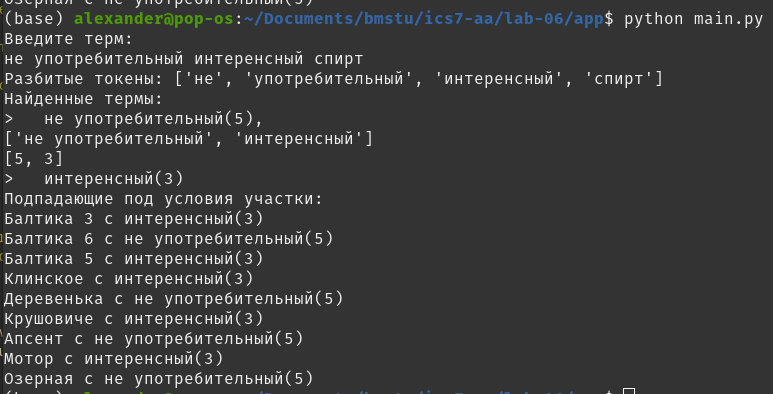
\includegraphics[scale=0.5]{assets/demon.png}
		\caption{Пример работы программы}
		\label{demonstration}
	\end{center}
	
	
\end{figure}

\newpage

\section{Время выполнения реализации алгоритмов}

Результаты замеров времени работы реализаций конвейерной линии приведены в таблице \ref{tbl:best}. 
Сравнение проводилось между простым алгоритмом и параллельного алгоритма при исполнении на 16 потоках.

\newcolumntype{d}[1]{D{.}{.}{-1}}
\begin{table}[ht!]
	\begin{center}
		\captionsetup{justification=raggedright,singlelinecheck=off}
		\caption{Замеры времени работы на очереди размером 18}
		\label{tbl:best}
	\begin{tabular}{|c|d{3.3}|d{3.3}|d{3.3}|d{3.3}|d{3.3}|d{3.3}|}
		\hline
		\multirow{3}{*}{№} & \multicolumn{6}{c|}{Начало обработки заявки} \\ \cline{2-7} 
		& \multicolumn{3}{c|}{Параллельно, мс.} & \multicolumn{3}{c|}{Синхронно, мс.} \\ \cline{2-7} 
		& Линия 1 & Линия 2 & Линия 3 & Линия 1 & Линия 2 & Линия 3 \\ \hline
		1   & 0          & 1.362      & 39.346     & 0          & 2.264     & 46.412      \\
		2   & 1.357      & 39.264     &   71.552   &   2.591    &   71.510    &  77.238  \\
		3   &   2.592    &  71.517    & 97.895     &   4.406    &   97.813   &  110.997    \\
		4   &   4.406   &   97.817   &   124.739   &  5.399    &  124.642    &  137.786   \\
		5   &   5.400   &  124.647    &  150.251    &   6.671   &  150.163    &  163.029    \\
		6   &   6.671   &  150.168    &  175.661    &  7.655    &  175.564    &  189.175    \\
		7   &   7.656   &  175.568    &   204.621   &  8.963    &   204.524   &   219.234   \\
		8   &   8.964   &   204.529   &  229.531    &   10.039   &   229.449   &   244.670   \\
		9   &   10.040   &   229.453   &   255.624   &  11.315    &  255.528    &  269.153    \\
		10  &   11.316   &   255.533   &   280.916   &   13.143   &  280.835    &  296.944    \\
		11   & 13.144   & 280.840      & 306.643    & 14.445   & 306.523    & 321.704      \\
		12   & 14.446     & 306.527    &   332.481   &   16.039    &   332.404    &   345.419    \\
		13   &    16.040   &  332.408    &  364.662    &   17.607    &   364.579   &   379.236   \\
		14   &   17.607   &  364.584    &    399.569  &   18.912   &  399.476    &   414.693   \\
		15   &    18.913  &   399.482   &    427.691  &   20.613   &   427.592   &   441.909   \\
		16   &   20.613   & 427.597     &  453.138    &  22.318    &   453.058   &  467.998    \\
		17   &  22.319    &   453.062   &   479.098   &  24.609    &   479.020   &  495.013    \\
		18   &  24.610    &   479.023   &   505.296   &   26.619   &   505.209   &  520.386    \\
		\hline
			\end{tabular}
\end{center}
\end{table}

Из таблицы можно сделать вывод, что распараллеленный конвейер выполняет работу на 10\% быстрее, чем синхронный.



\section*{Вывод}

В данном разделе были сравнены алгоритмы по времени.
Выявлено, что конвейерная обработка быстрее последовательной на 10\% (2 мс. при размере матрицы 100 на 100). 
 
